%=======================02-713 LaTeX template, following the 15-210 template==================
%
% You don't need to use LaTeX or this template, but you must turn your homework in as
% a typeset PDF somehow.
%
% How to use:
%    1. Update your information in section "A" below
%    2. Write your answers in section "B" below. Precede answers for all 
%       parts of a question with the command "\question{n}{desc}" where n is
%       the question number and "desc" is a short, one-line description of 
%       the problem. There is no need to restate the problem.
%    3. If a question has multiple parts, precede the answer to part x with the
%       command "\part{x}".
%    4. If a problem asks you to design an algorithm, use the commands
%       \algorithm, \correctness, \runtime to precede your discussion of the 
%       description of the algorithm, its correctness, and its running time, respectively.
%    5. You can include graphics by using the command \includegraphics{FILENAME}
%
\documentclass[11pt]{article}
\usepackage{amsmath,amssymb,amsthm}
\usepackage{graphicx}
\usepackage[margin=1in]{geometry}
\usepackage{fancyhdr}
\usepackage{listings}
\usepackage{float} 
\usepackage{subfig}
\usepackage{pdfpages}

\setlength{\parindent}{0pt}
\setlength{\parskip}{5pt plus 1pt}
\setlength{\headheight}{13.6pt}
\newcommand\question[2]{\vspace{.25in}\hrule\textbf{#1: #2}\vspace{.5em}\hrule\vspace{.10in}}
\renewcommand\part[1]{\vspace{.10in}\textbf{(#1)}}
\newcommand\algorithm{\vspace{.10in}\textbf{Algorithm: }}
\newcommand\ot{\vspace{.10in}\textbf{Output: }}
\newcommand\runtime{\vspace{.10in}\textbf{Running time: }}
\pagestyle{fancyplain}
\lhead{\textbf{\NAME\ (\ANDREWID)}}
\chead{\textbf{Lab\HWNUM}}
\rhead{\today}
\begin{document}\raggedright
%Section A==============Change the values below to match your information==================
\newcommand\NAME{Yao Xiao}  % your name
\newcommand\ANDREWID{2019180015}     % your andrew id
\newcommand\HWNUM{8}              % the homework number
%Section B==============Put your answers to the questions below here=======================

% no need to restate the problem --- the graders know which problem is which,
% but replacing "The First Problem" with a short phrase will help you remember
% which problem this is when you read over your homeworks to study.

\question{1}{The First Problem} 

\part{a} \algorithm
\begin{lstlisting}
import numpy as np
from sko.GA import GA
import pandas as pd
import matplotlib.pyplot as plt

def schaffer(p):
    x, = p
    return x + 10 * np.sin(x) + 7 * np.cos(x)

ga = GA(func=schaffer, n_dim=1, size_pop=50, max_iter=1000, lb=[0], ub=[10], precision=1e-07)
best_x, best_y= ga.run()

Y_history = pd.DataFrame(ga.all_history_Y)
fig, ax = plt.subplots(2, 1)
ax[0].plot(Y_history.index, Y_history.values, '.', color='red')
Y_history.min(axis=1).cummin().plot(kind='line')
plt.show()
\end{lstlisting}

\part{b} \ot

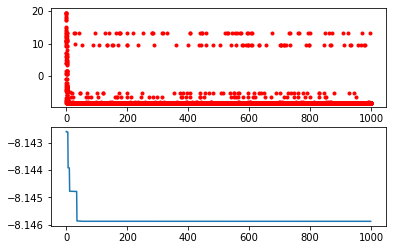
\includegraphics{Fig1.png}


\question{2}{The Second Problem}

\part{a} \algorithm
\begin{lstlisting}
import numpy as np
from sko.GA import GA
import pandas as pd
import math 
import matplotlib.pyplot as plt

def schaffer(p):
    x,y = p
    return y * np.sin(2*math.pi * x) + x * np.cos(2 * math.pi * y)

ga = GA(func=schaffer, n_dim=2, size_pop=50, max_iter=1000, lb=[-2,-2], ub=[2,2], precision=1e-05)
best_x, best_y= ga.run()

Y_history = pd.DataFrame(ga.all_history_Y)
fig, ax = plt.subplots(2, 1)
ax[0].plot(Y_history.index, Y_history.values, '.', color='red')
Y_history.min(axis=1).cummin().plot(kind='line')
plt.show()
\end{lstlisting}

\part{b} \ot

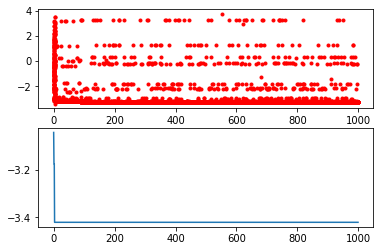
\includegraphics{Fig2.png}

\end{document}
